\documentclass{article}\usepackage[margin=20mm]{geometry}\usepackage{graphicx,booktabs}\begin{document}\title{MC selection}\author{}\date{\today}\maketitle
Requested 5,000 catalogue events per sample; processed 1,657 double-beta and 1,552 electron events (limited by available input events). Independent samples, no event matching. Source coordinates, all particles, no diffusion or fiducial cut. Voxel threshold is inclusive and precedes graph construction. Accept exactly one connected component, including a one-node component. Event track length is the longest component backbone. Voxel-energy and component-length histograms pool entries over events; all other histograms have one entry per event. After-selection histograms use the same quantities and bins as before selection. Efficiencies include binomial standard errors and z=1 Wilson intervals. Float32 is used for physical reductions; saved Float64 sums provide independent precision references. Timing excludes initial Julia startup from serial warm-up; warm-up uses one event. Parallel uses two separate Julia processes with owned HDF5 readers, warmed behind a start barrier. Parallel batch time includes dispatch, reading, calculation and shard writing. Parallel total additionally includes process startup and warm-up. Each sample is benchmarked serial first; OS caches may favour the subsequent parallel run. Numerical output is the serial reference.

distance\_mode = voxel\_multiple\\
distance\_voxel\_multiple = 2.5\\
energy\_threshold\_keV = 1.0\\
k = 10\\
max\_distance\_mm = 1.25\\
method = KDT\\
voxel\_width\_mm = 0.5
\section*{Selection efficiency}\begin{center}\resizebox{\linewidth}{!}{\begin{tabular}{lllll}\toprule Sample & Processed & Accepted & Efficiency [\%] & Wilson 68\% [\%]\\\midrule 
Double beta (100 $\mu$m) & 1657 & 680 & 41.0 $\pm$ 1.2 & [39.8, 42.3]\\
Single electrons (100 $\mu$m) & 1552 & 619 & 39.9 $\pm$ 1.2 & [38.6, 41.1]\\\bottomrule\end{tabular}}\end{center}
\section*{Energy validation}\begin{center}\resizebox{\linewidth}{!}{\begin{tabular}{llll}\toprule Sample & Max energy closure [keV] & Max voxel error vs Float64 [keV] & Serial/parallel identical\\\midrule 
Double beta (100 $\mu$m) & 0.000954 & 0.000734 & True\\
Single electrons (100 $\mu$m) & 0.000954 & 0.000772 & True\\\bottomrule\end{tabular}}\end{center}
\section*{Timing}
Double beta (100 $\mu$m)\begin{itemize}
\item Serial warm-up [s]: 3.003
\item Read [s]: 2.487
\item Analysis [s]: 4.333
\item Serial batch [s]: 6.824
\item 2-process batch [s]: 3.998
\item Process startup + warm-up [s]: 5.931
\item Parallel total [s]: 9.929
\end{itemize}
Single electrons (100 $\mu$m)\begin{itemize}
\item Serial warm-up [s]: 0.005
\item Read [s]: 2.118
\item Analysis [s]: 4.239
\item Serial batch [s]: 6.357
\item 2-process batch [s]: 3.772
\item Process startup + warm-up [s]: 5.933
\item Parallel total [s]: 9.705
\end{itemize}
\clearpage\section*{Occupied voxel energy}\noindent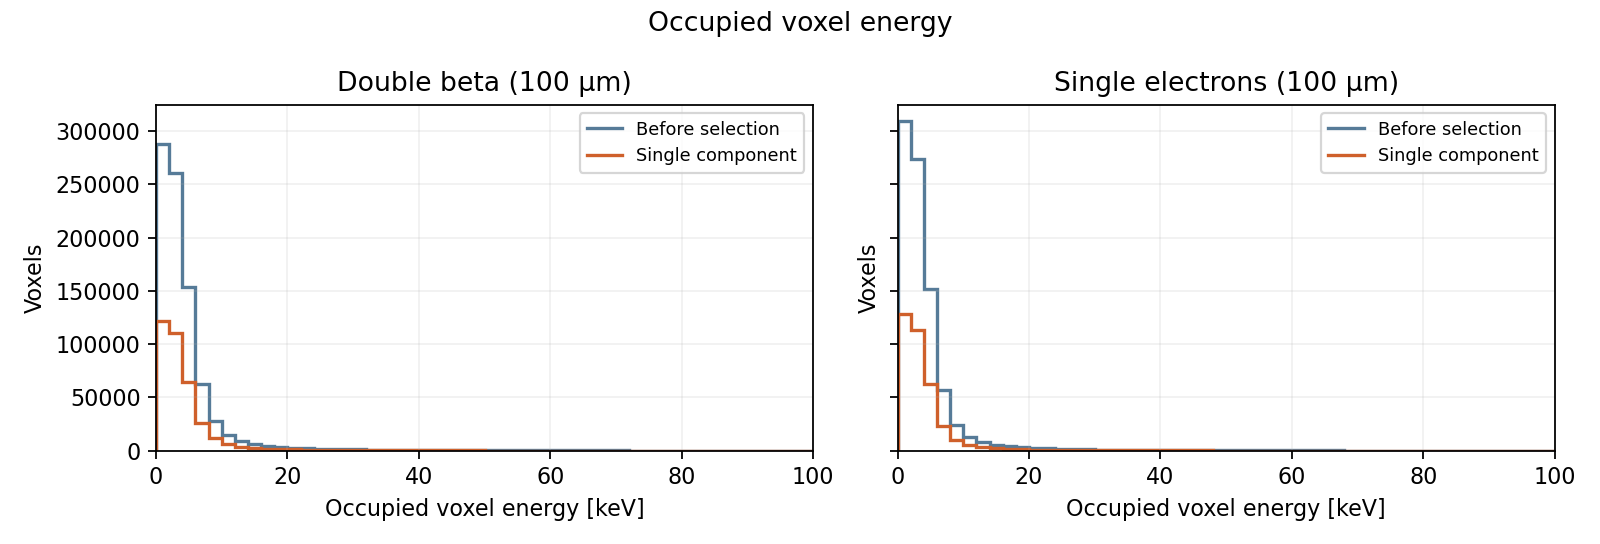
\includegraphics[width=\linewidth]{voxel_energy_MeV.png}

Double beta (100 $\mu$m): before under/overflow 0/0, after 0/0; Single electrons (100 $\mu$m): before under/overflow 0/0, after 0/0
\clearpage\section*{Occupied voxels per event}\noindent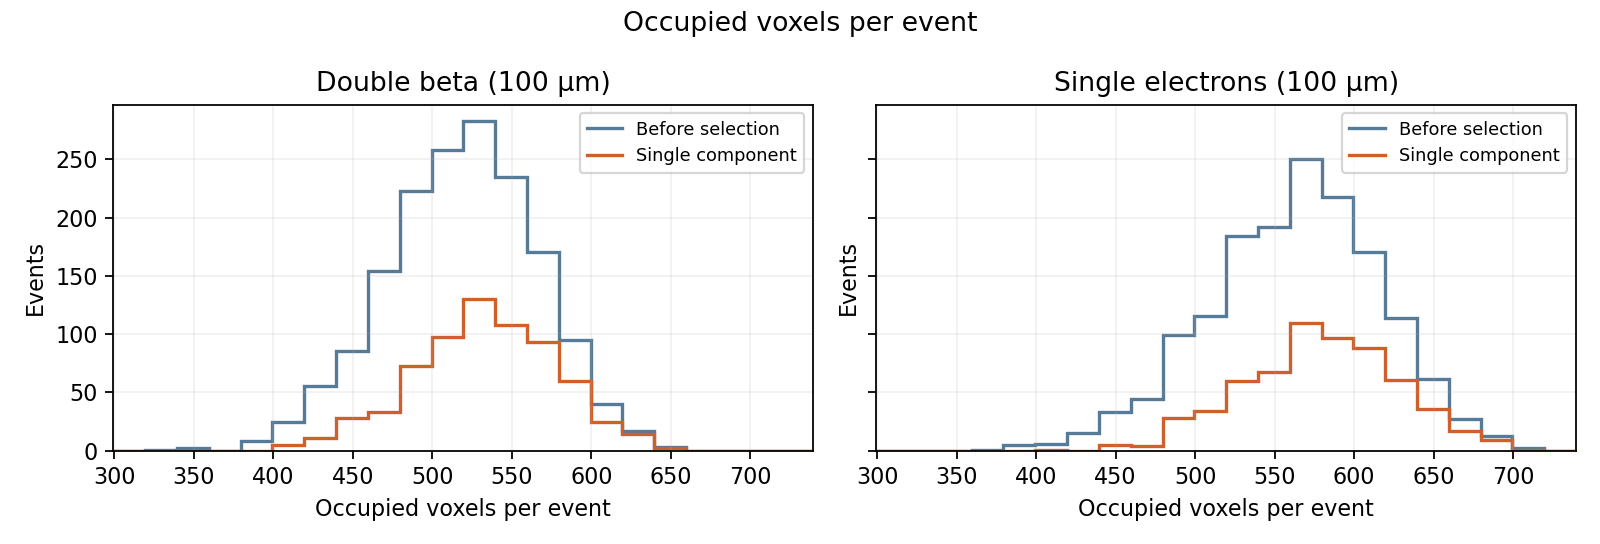
\includegraphics[width=\linewidth]{n_voxels.png}

Double beta (100 $\mu$m): before under/overflow 0/0, after 0/0; Single electrons (100 $\mu$m): before under/overflow 0/0, after 0/0
\clearpage\section*{Longest component backbone}\noindent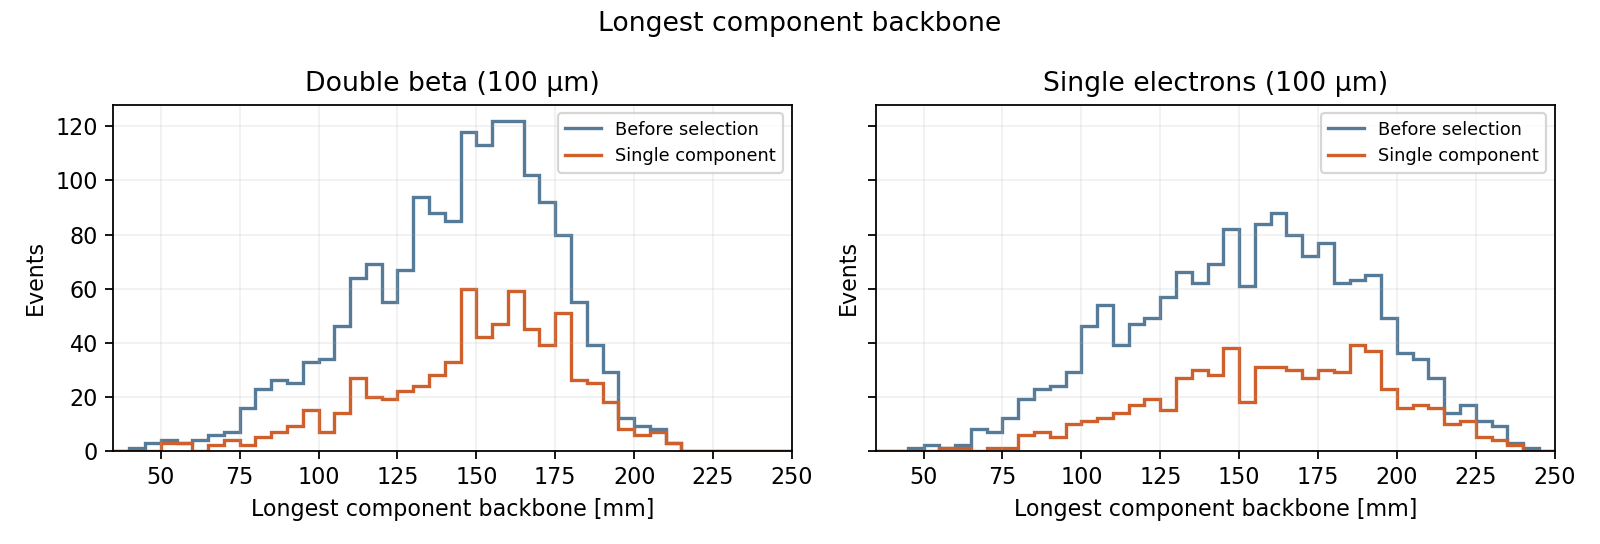
\includegraphics[width=\linewidth]{track_length_mm.png}

Double beta (100 $\mu$m): before under/overflow 0/0, after 0/0; Single electrons (100 $\mu$m): before under/overflow 0/0, after 0/0
\clearpage\section*{Total voxel energy per event}\noindent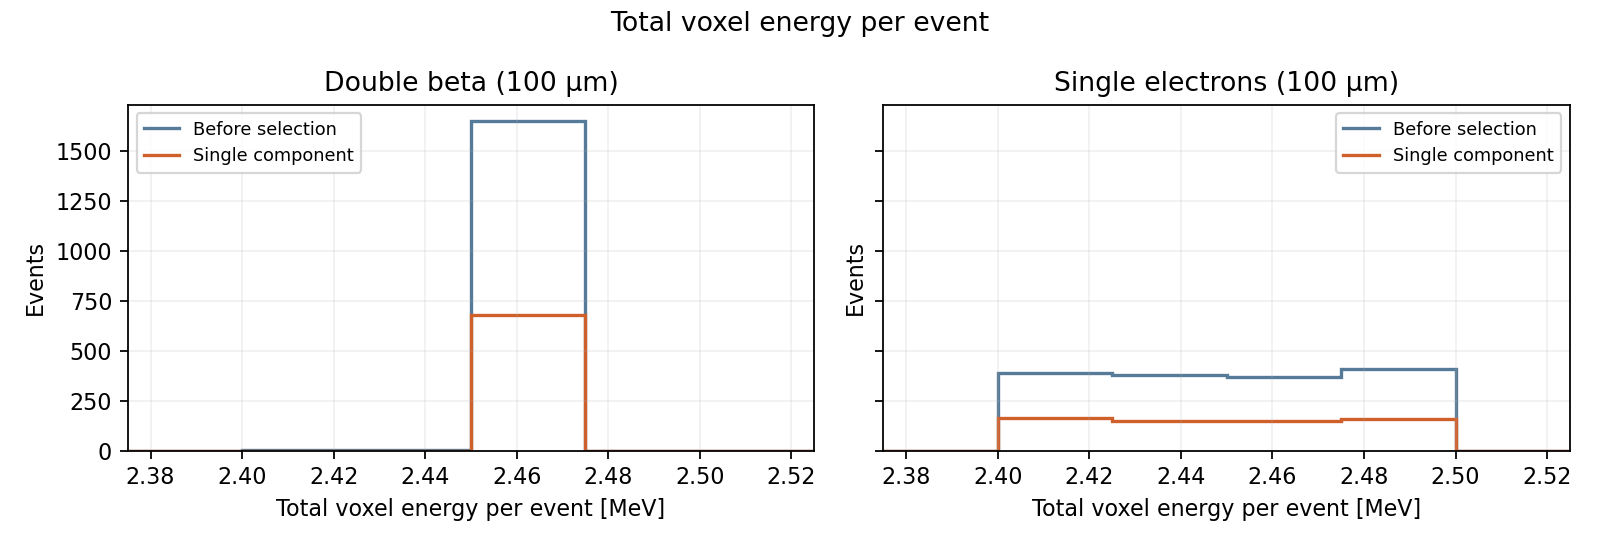
\includegraphics[width=\linewidth]{voxel_energy_sum_MeV.png}

Double beta (100 $\mu$m): before under/overflow 0/0, after 0/0; Single electrons (100 $\mu$m): before under/overflow 0/0, after 0/0
\clearpage\section*{Connected components per event}\noindent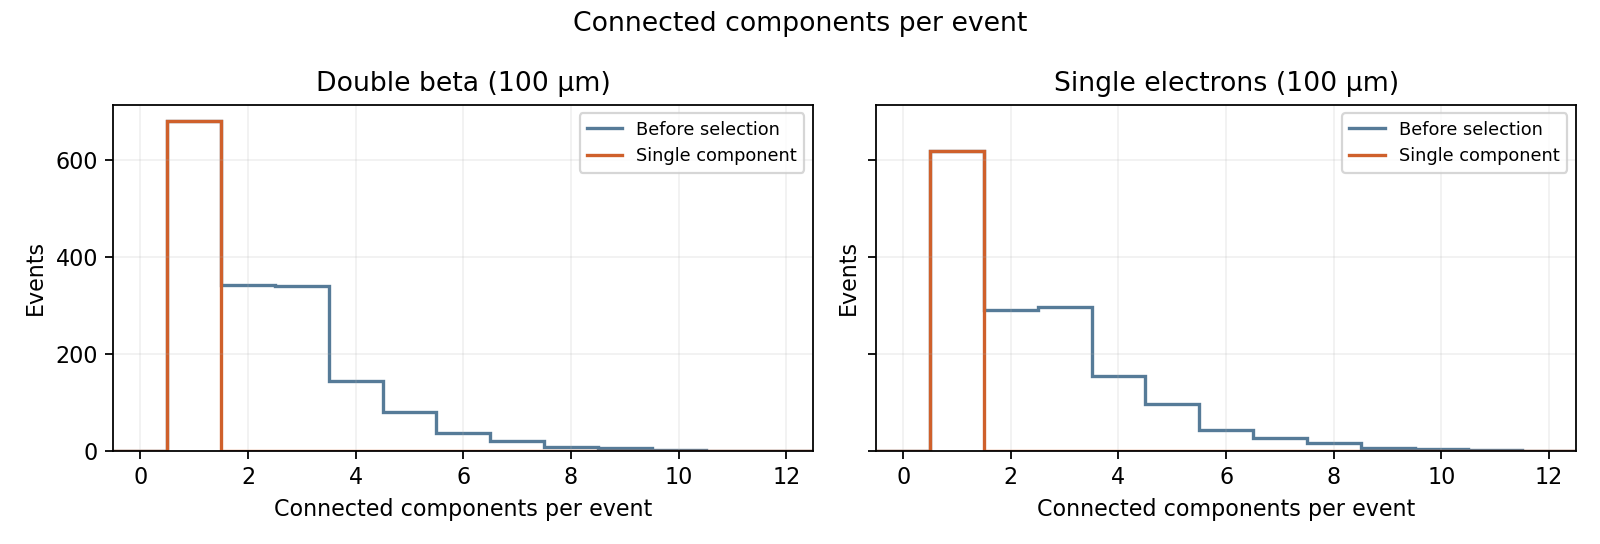
\includegraphics[width=\linewidth]{n_components.png}

Double beta (100 $\mu$m): before under/overflow 0/0, after 0/0; Single electrons (100 $\mu$m): before under/overflow 0/0, after 0/0
\clearpage\section*{Voxel energy after threshold}\noindent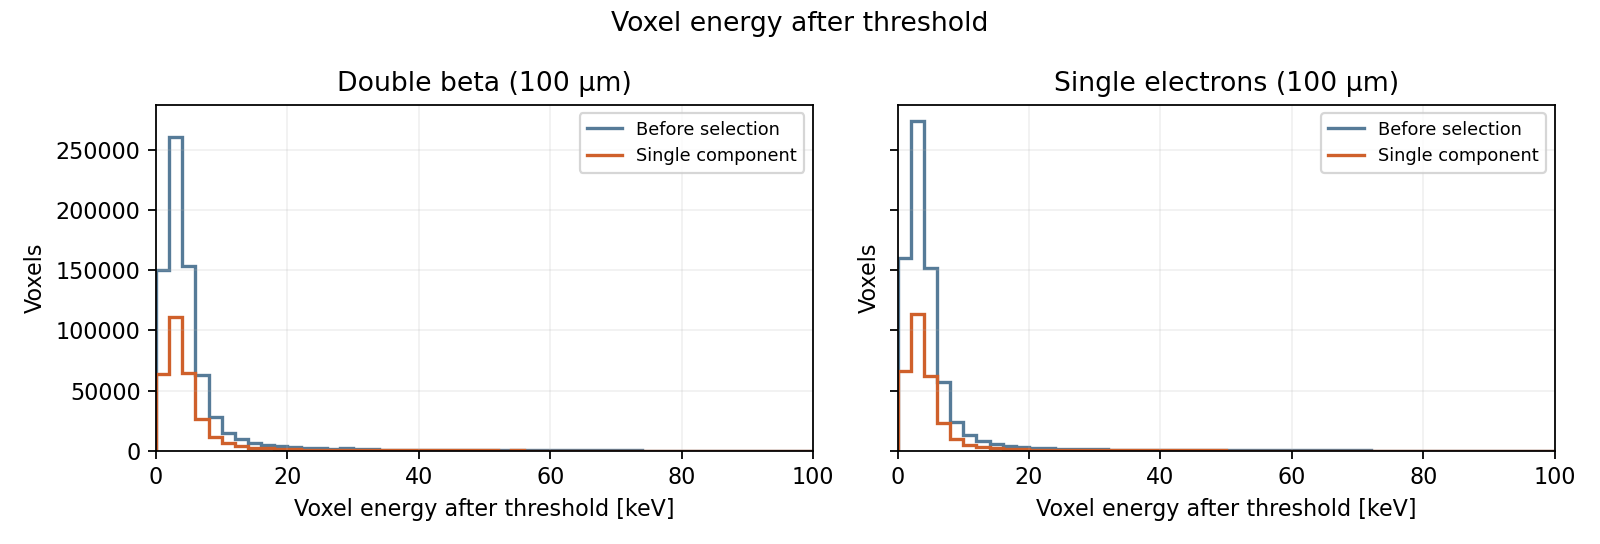
\includegraphics[width=\linewidth]{retained_voxel_energy_MeV.png}

Double beta (100 $\mu$m): before under/overflow 0/0, after 0/0; Single electrons (100 $\mu$m): before under/overflow 0/0, after 0/0
\clearpage\section*{Voxels after threshold per event}\noindent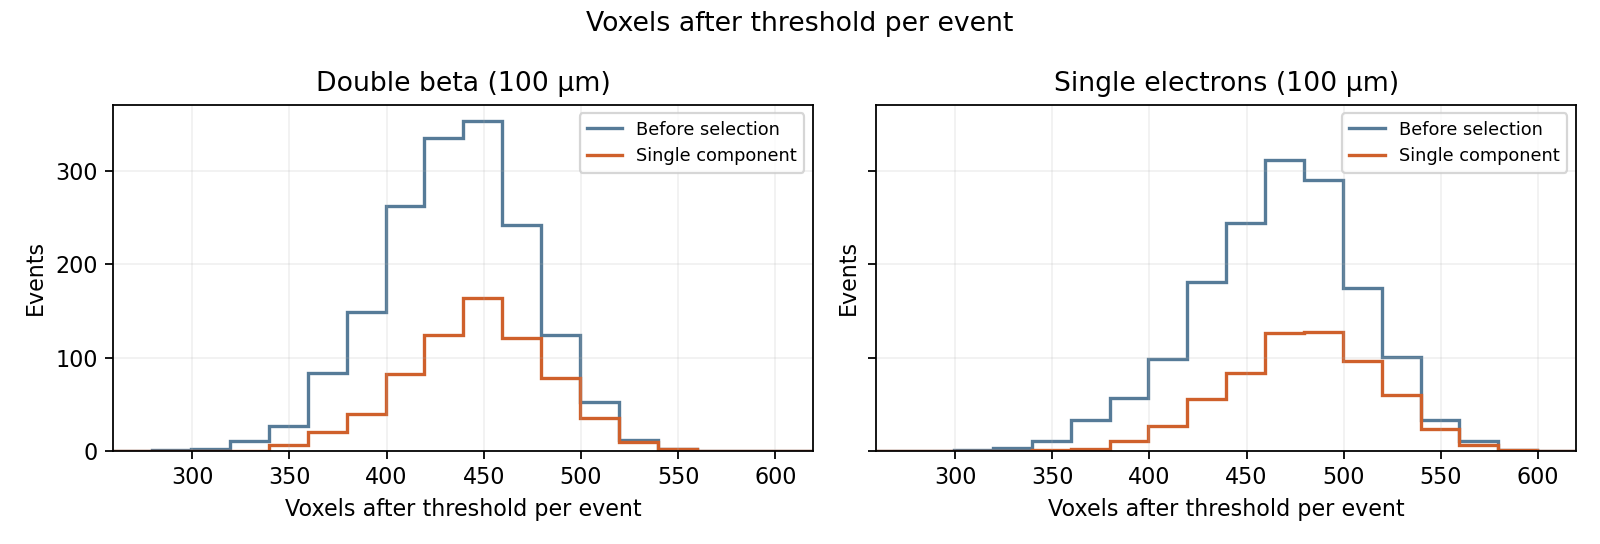
\includegraphics[width=\linewidth]{n_retained_voxels.png}

Double beta (100 $\mu$m): before under/overflow 0/0, after 0/0; Single electrons (100 $\mu$m): before under/overflow 0/0, after 0/0
\clearpage\section*{Graph-retained energy per event}\noindent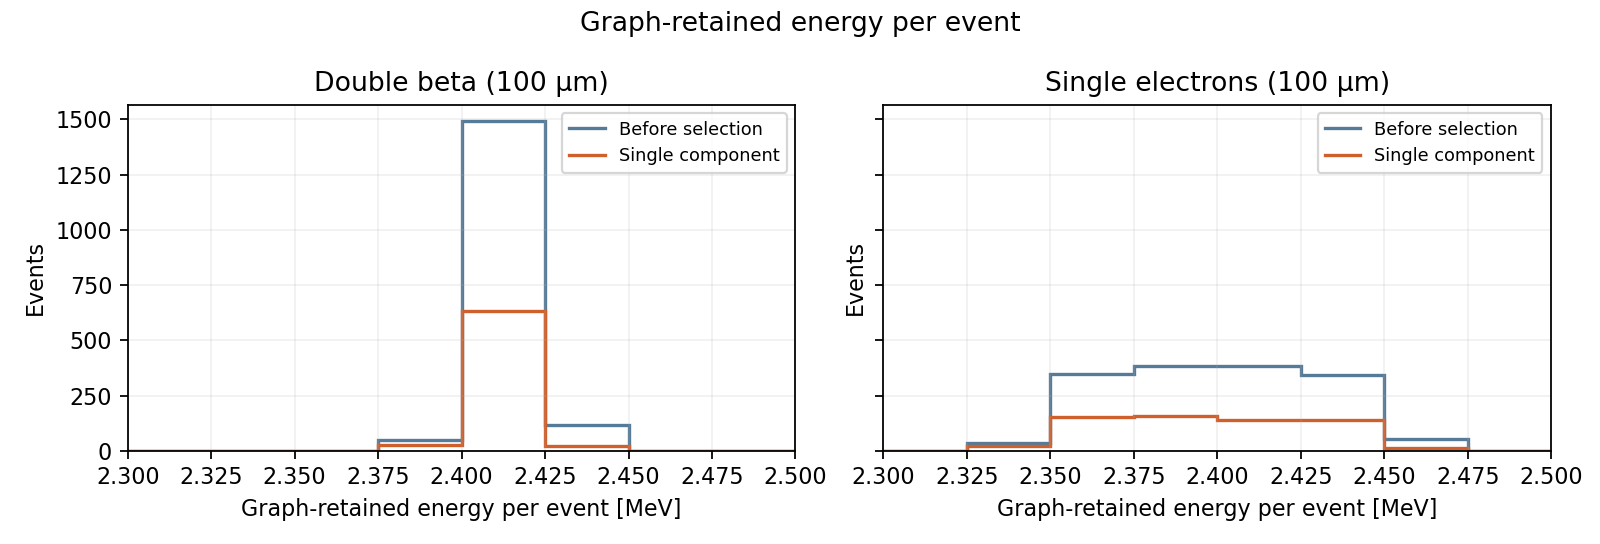
\includegraphics[width=\linewidth]{retained_energy_sum_MeV.png}

Double beta (100 $\mu$m): before under/overflow 0/0, after 0/0; Single electrons (100 $\mu$m): before under/overflow 0/0, after 0/0
\clearpage\section*{Individual component backbones}\noindent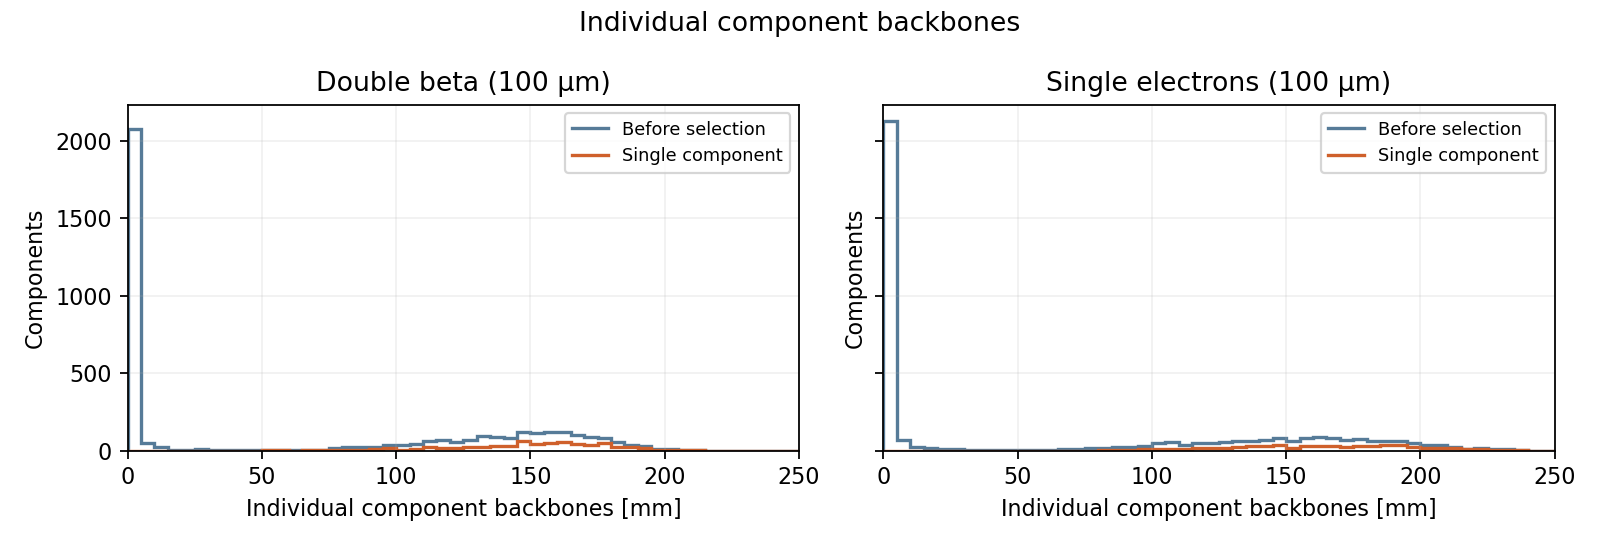
\includegraphics[width=\linewidth]{component_length_mm.png}

Double beta (100 $\mu$m): before under/overflow 0/0, after 0/0; Single electrons (100 $\mu$m): before under/overflow 0/0, after 0/0
\end{document}